% -*- mode: fundamental -*-

% ****************************************************************

\chapter{{\BSV}: Combinational circuits for the RISC-V Stage functions}

\markboth{Ch \arabic{chapter}: Combinational functions (DRAFT)}{\copyrightnotice}

\setcounter{page}{1}
% \renewcommand{\thepage}{\arabic{page}}
\renewcommand{\thepage}{\arabic{chapter}-\arabic{page}}

\label{ch_Combo_Circuits}

% ****************************************************************

\section{Introduction}

It is useful to start with the Decode stage of
Figure~\ref{Fig_Instr_Exec} because it involves only bit-vectors,
operations on bit-vectors, conditionals to classify instructions into
classes, and \verb|enum| types to name and encode instruction classes.

The inputs to the Decode stage as depicted in the diagram are:

\begin{tightlist}

 \item A 32-bit piece of data---a RISC-V instruction---that has become
 available by reading it from memory at the PC address.\footnote{When
 implementing the so-called ``C'' RISC-V ISA extension (``compressed
 instructions''), instructions can also be 16 bits, but we ignore that
 for RV32I.}

 \item Any additional information passed on from the Fetch stage.

\end{tightlist}

The outputs of the Decode stage have information needed by the next
stage (Register-Read and Dispatch).  For a RISC-V instruction, useful
information includes:

\begin{tightlist}

 \item Was the Fetch itself successful, or did it encounter a memory
   error; if so, what kind of memory error?

 \item Is it a legal 32-bit instruction?

 \item If legal, what is its broad classification: Control (Branch or
   Jump)? Integer Arithmetic or Logic? Memory Access?  This will help
   in choosing the next stage to which we must dispatch to execute the
   instruction.

 \item Does it have zero, one or two input registers?  If so, which
   ones?  This will help the next stage in reading registers.

 \item Does it have zero or one output registers?  If so, which one?
   This will help the final Register Write stage in writing back a
   value to a register.

\end{tightlist}

To compute these values, we need to examine ``slices'' of the 32-bit
instruction (``bit vector''), such as the 7-bit ``opcode'' slice, the
5-bit ``rs1'', ``rs2'' and ``rd'' slices, and so on.  We need to be
able to compare these slices to constants ({\eg} ``Is the opcode a
BRANCH opcode?'').  We need to do things conditionally, {\eg} if it is
a BRANCH instruction, then it has an rs1 and rs2 slice but no rd
slice, but if it is a JAL instruction it has an rd slice but no rs1 or
rs2.  Finally, as in any good programming language, we need to package
all this functionality inside ``functions'' with clearly specified
input(s) and output(s).  In the next several sections we will learn
the {\BSV} concepts needed to code these ideas.

% ****************************************************************

\section{Hexadecimal and Binary Notation for literal integers}

\label{BSV_hex_bin_literals}

\index[BSV]{Literals!Hexadecimal integer notation}
\index[BSV]{Literals!Binary integer notation}
\index[BSV]{Hexadecimal notation for integer literals}
\index[BSV]{Binary notation for integer literals}

{\BSV} uses the same notation as Verilog and SystemVerilog for
hexadecimal and binary literal integers.  Some examples:

{\footnotesize
\begin{Verbatim}[frame=single, numbers=left]
3'b010            // Binary literal, 3 bits wide
7'b_110_0011      // Binary literal, 7 bits wide
5'h3              // Hex literal, 5 bits wide
32'h3             // Hex literal, 5 bits wide
32'h_efff_0f17    // Hex literal, 32 bits wide (an AUIPC instruction)
'h23              // Hex literal, context determines width
\end{Verbatim}
}

As these examples show, a hexadecimal or binary integer literal is
introduced by an optional bit-width, then a ``tick'' (single-quote)
character, and then the binary or hexadecimal digits for the number.
The character ``{\verb|_|}'' may be used freely to space out groups of
digits to improve readability for humans (the compiler ignores these
spacers).

The last line shows that we can omit the size prefix, in which case
the size will be inferred by the compiler from the context. For
example, if we had:

{\footnotesize
\begin{Verbatim}[frame=single]
   Bit #(32) pc_val = 'h_8000_0000;
\end{Verbatim}
}

then the literal is inferred to be 32 bits wide, and this will be
extended, if necessary to fit the context where it is used.

% ****************************************************************

\section{Syntax of Identifiers}

\label{BSV_Syntax_of_Identifiers}

\index[BSV]{Identifer syntax}

The syntax of an identifier (name) in {\BSV} follows the same conventions
as in many programming languages: any sequence of alphabets, digits
and underscore characters, with the first letter always being an
alphabet.

\index[BSV]{Identifiers!First letter lower- or uppercase}
\index[BSV]{Identifiers!Type: initial uppercase letter}
\index[BSV]{Identifiers!Enum constant: initial uppercase letter}
\index[BSV]{Identifiers!Ordinary: initial lowercase letter}

{\BSV} follows the Haskell system where an identifier has a different
role depending on whether its first letter is uppercase or lowercase.
An uppercase first letter names a \emph{constant}, either a value
constant or a type constant.  A lowercase first letter names a
\emph{variable}, either a value variable or a type variables.

\index[BSV]{True@{\tt True} ({\tt Bool} constant)}
\index[BSV]{False@{\tt False} ({\tt Bool} constant)}

The identifiers \verb|True| and \verb|False| are predefined value
constants (they begin with an uppercase letter) representing standard
boolean values.  In the enum type-definition in
Section~\ref{BSV_enum_types}, the identifiers \verb|OPCLASS_SYSTEM|,
\verb|OPCLASS_CONTROL|, \verb|OPCLASS_INT| and \verb|OPCLASS_MEM| are
also value constants.

The identifiers \verb|Bool| and \verb|Bit| are predefined type
constants.  In the enum type-definition in
Section~\ref{BSV_enum_types}, the identifier \verb|OpClass| is a type
constant.\footnote{The identifiers {\tt Bits}, {\tt Eq}, and {\tt
FShow} are all predefined ``typeclass'' constants.  Typeclasses are an
somewhat advanced topic which we will not be discussing much in this
book beyond the brief mention in Section~\ref{Sec_Typeclasses}.  }

Other identifiers in the following sections, like \verb|pc_val|,
\verb|x|, \verb|y|, \verb|a|, \verb|b|, \verb|opcode|, and
\verb|funct3| are all ordinary value variables (begin with a lowercase
letter).  Even function names, such as \verb|instr_funct3| and
\verb|is_legal_BRANCH| are value variables.

Type variables are only used in so-called \emph{polymorphic} types and
functions, where a single function is defined to work over a family of
types.  For example we can write a function to exchange the order of
bits in a bit-vector of any width; its argument and result types would
be given as \verb|Bit#(n)|, where \verb|n| is a type variable.

% ****************************************************************

\section{Syntax of comments}

\label{BSV_Syntax_of_comments}

\index[BSV]{Comments!to end-of-line, starting with {\tt //}}
\index[BSV]{Comments!block, from {\tt /*} to matching {\tt */}}
\index[BSV]{//@{\tt //}, start of comment-to-end-of-line}
\index[BSV]{/*@{\tt /*}, start of block comment (until-{\tt */})}

Comments in {\BSV} have the same syntactic conventions as in Verilog,
SystemVerilog and C/C++:

\begin{itemize}

  \item A pair of forward-slashes (``\verb|//|'') begins a comment
    (text ignored by {\bsc}) that spans to the end of the current
    line.  There are many examples of this in the code fragments
    already shown above.

  \item A region of text, possibly spanning multiple lines, is a
    comment (ignored by {\bsc}) if preceded by ``\verb|/*|'' and
    followed by ``\verb|*/|''.  This is often used to ``comment-out''
    regions of text during debugging or trying out alternatives, and
    for long documentation notes.

\end{itemize}

% ****************************************************************

\section{Introduction to Types}

\label{Sec_Types_Intro}

\index[BSV]{Data types}
\index[BSV]{Types (data types; sets of values)}

\index[BSV]{Numeric Kind}
\index[BSV]{Value Kind}

\index[BSV]{Kinds!Numeric}
\index[BSV]{Kinds!Value}

Like all \emph{safe} modern programming languages, {\BSV} has an
expressive type system and is strongy typechecked.

By \emph{expressive} type system we mean that it has a rich vocabulary
for organizing values: booleans, bit-vectors, signed integers, enums,
structs, vectors, functions, actions, rules, modules and more.  By
\emph{strongly typechecked} we mean that there are strict compile-time
rules about what types of arguments are allowed for each operator or
function, and what type of result they produce.  These rules disallow
misinterpretatio of values, mistakes like taking the square-root of an
ASCII character, or extracting the struct field from something that
does not represent a struct.  Types are \emph{language-level
abstractions}: ultimately both software and hardware compute with raw
bits, but a language's type-system and type-checking ensure that bits
are organized and used in intended ways.

{\BSV}'s type-checking rules go beyond most programming languages by also
\emph{checking many size constraints}.  For example, a {\BSV} function
that expects a bit-vector of width exactly 32 bits cannot be given a
bit-vector of any other size.  In many other languages, they will
silently extend a narrower argument or truncate a wider argument to
the expected size; that behavior is very dangerous in hardware design,
where we work with scalar values of many, many different
precisely-sized bit-widths, unlike software languages where we
typically use a bit-width that is generously large enough to
accommodate our scalar values (8, 16, 32, 64 bits).

Figure~\ref{Fig_BSV_Types} illustrates the type hierarchy in {\BSV}.
\begin{figure}[htbp]
  \centerline{\includegraphics[width=\textwidth,angle=0]{Figures/Fig_BSV_Types}}
  \caption{\label{Fig_BSV_Types}The hierarchy of Values, Types and Kinds}
\end{figure}
The lower two layers are quite conventional: Types represent sets of
Values.  The upper-layer (Kinds) expresses the idea that within a type
expression (middle layer), certain components of the type-expression
(shown in red) are of \emph{Numeric Kind}, representing some ``size''
feature of the type.

% ----------------
\vspace{1ex}

NOTE: \fbox{\small
\begin{minipage}{5in}

{\bf About numeric kinds:} Even though we use numeric notation like
``3'' and ``16'' both at the value level and at the type level, these
two uses are completely distinct.  They occur in distinct
contexts---value expressions {\vs} type expressions---and so there is
no ambiguity.

\vspace{1ex}

Numeric types are all known to {\bsc} at compile time whereas, of
course, numeric values are computed and used dynamically during
execution.

\vspace{1ex}

\index[BSV]{valueOf@{\tt valueOf} pseudo-function from numeric types to numeric values}
\index[BSV]{Types!valueOf@{\tt valueOf}: value of a numeric type}

There is a {\BSV} pseudo-function {\tt valueOf($t_{numeric}$)} which,
given a numeric type $t_{numeric}$, produces the numeric \emph{value}
corresponding to $t_{numeric}$.  This is feasible because
$t_{numeric}$ is statically known to {\bsc}.  It does not make sense
to have a function in the opposite direction, from numeric values to
numeric types, because one cannot compute something static from a
dynamic value.  {\tt valueOf($t_{numeric}$)} is a pseudo-function and
not a normal function because its ``argument'' is a type, not a value.

\vspace{1ex}

We can of course perform arbitrary arithmetic on numeric values
because they are dynamic.

\vspace{1ex}

We can perform only limited forms of arithmetic on numeric types
because they have to be evaluted statically by {\bsc}.  Consider a
generic function that takes two arguments of type {\tt Bit\#(m)} and
{\tt Bit\#(n)} and returns the concatenation of these bit-vectors: its
output type is {\tt Bit\#(m+n)}.  By limiting the available arithmetic
\emph{bsc} can resolve it statically.  This is a somewhat advanced
topic which we postpone until Section~\ref{Sec_Typeclasses}.

\end{minipage}}

\vspace{1ex}
% ----------------

Types can nested to arbitrary depth:

\begin{tabbing}
 \hmmmm \emph{type} ::= \emph{type-constructor} {\tt \#(} \emph{type}, ..., \emph{type} {\tt )}
\end{tabbing}

A \emph{type-constructor} always begins with an upper-case letter (is a type constant).

For each \emph{type-constructor}, each \emph{type} argument
(parameter) is fixed to be either of value kind or numeric kind.

For example,

\begin{itemize}

 \item In \verb|Bit #(n)|, \verb|n| is always of numeric kind.

 \item In \verb|Vector #(n,t)|, \verb|n| is always of numeric kind,
 \verb|t| is always of value kind.

 \item In \verb|Tuple3 #(t1,t2,t3)|, all three parameters are always of value kind.

\end{itemize}

Note that \verb|Bit#(3)| and \verb|Int#(3)|, although both represented
in hardware with 3 bits, are distinct types.  The former can represent
values in the range 0..7; the latter in the range -4..3.
\verb|Bit#(3)| is a distinct type from \verb|Bit#(4)|.  2-tuples
(pairs of values of heterogeneous types) are distinct from 3-tuples.
4-element vectors are a distinct type from 2-element vectors.

% ****************************************************************

\section{Bit vectors, and declaring identifiers}

\label{Sec_BSV_Bit_Vectors}

\index[BSV]{Bit Vectors}
\index[BSV]{Types!{\tt Bit\#(n)}}

The simplest, and lowest-level type in {\BSV} is the bit-vector (a vector
made up of a particular number bits).  It is ``lowest-level'' in that
it is the only type that directly maps into hardware and can be
observed directly in hardware with a waveform viewer or an
oscilloscope.  Later we will see that in {\BSV} one can define more
abstract types such as integers, booleans, vectors and arrays, lists,
structs (records), tagged unions (algebraic types), trees, and so on.
These are all language-level abstractions, {\ie} a language-level view
of bits; ultimately, all values are represented in hardware as
bit-vectors.

The {\BSV} statement:

{\footnotesize
\begin{Verbatim}[frame=single, numbers=left]
   Bit #(32) pc_val = 32'h_8000_0000;
\end{Verbatim}
}

declares the identifier \verb|pc_val| to have the type
\verb|Bit#(32)|, {\ie} a bit-vector of 32 bits, and initializes it to
have the value shown in hexadecimal on the right-hand side.

The general syntax is similar to C or Verilog:
\begin{quote}
\emph{type} \emph{identifier} = \emph{initial\_value};
\end{quote}

The BSC type \verb|Bit#(32)| is roughly equivalent to the C type
\verb|uint32_t|.  Unlike C, where only a few sizes are available, all
multiples of 8 bits--- (\verb|uint8_t|, \verb|uint16_t|,
\verb|uint32_t| and \verb|uint64_t|)---bit-vectors in {\BSV} can have any
size (\verb|Bit#(3)|, \verb|Bit#(51)|, \verb|Bit#(512)|, ...).

The initial value's size can be left unspecified:

{\footnotesize
\begin{Verbatim}[frame=single, numbers=left]
   Bit #(32) pc_val = 'h_1000;
\end{Verbatim}
}

{\bsc} will infer that it should be 32 bits, and will zero-extend
accordingly.  If the constant is too large for the context, {\bsc}
will not silently truncate it; it will give an error-message instead.

% ================================================================

\subsection{Don't-care values} 

\label{Sec_Dont_Care_Values}

\index[BSV]{Don't care literal value {\tt ?}}
\index[BSV]{?@{\tt ?} (don't care literal value)}
\index[BSV]{AAAA\_AAAA@{\tt AAAA\_AAAA}, the default don't care value}

If the identifier will be assigned later, you can indicate that you
don't care about its initial value, like this:

\begin{quote}
\emph{type} \emph{identifier} = {\tt ?};
\end{quote}

``Don't care'' values are useful for several reasons.  First, this
conveys to the human reader that the value here is irrelevant.

Second, it can result in more efficient circuitry.  If we had said
``0'', for example, the \emph{bsc} compiler has to create circuitry
ensuring that field's value is 0. By saying ``\verb|?|'', the
\emph{bsc} compiler is allowed to pick any value that minimizes
circuitry.

Third, in places where it does not result in additional hardware, the
\emph{bsc} compiler usually injects the specific value
\verb|'h_AAAA_AAAA| (of suitable bit-width).  While debugging,
observing such a value in some computation is often a clue that
something is wrong.

\vspace{2ex}
% ----------------

\index[BSV]{X values!Notation for unassigned values in Verilog (no such concept in BSV)}

NOTE: \fbox{\small
\begin{minipage}{5in}

Verilog, SystemVerilog and VHDL have a concept of ``X'' values.  Each
bit of a register or wire carries an ``X'' value until it has been
assigned a specific binary value (0 or 1).  However, note that this is
\emph{only in simulation}, where the simulator can and does model
3-valued logic (0, 1 and X) for each bit, and is able to propagate X
values through operators, registers, {\etc} Hardware only implements
2-valued logic---every bit is either 0 or 1. Thus, this is an artefact
that is only useful during debugging in simulation and static
analysis.

\vspace{1ex}

BSV only has 2-valued logic; there is no concept of an ``X'' value.  A
BSV ``{\tt ?}'' expression has some specific, but potentially
unpredictable, binary value.

\end{minipage}}
% ----------------
\vspace{2ex}

% ----------------------------------------------------------------
\Beginexercise

Please see directory: \hm {\tt Exercises/Ex\_04\_A\_Bit\_Vectors/} \\
and its README.
\Endexercise

% ================================================================

\subsection{Built-in Operators on Bit Vectors}

\label{Bit_Vector_Ops}

The bits in a {\BSV} bit-vector of size $n$ are indexed from $n-1$
(most-significant bit) to 0 (least-significant bit).  You can extract
a \emph{slice} of a bit-vector using usual Verilog notation:

\index[BSV]{Bit Vectors!slices of}

{\footnotesize
\begin{Verbatim}[frame=single, numbers=left]
   Bit #(12) page_offset = pc_val [11:0];
   Bit #(1)  pc_lsb      = pc_val [0];
   Bit #(1)  pc_msb      = pc_val [31];
\end{Verbatim}
}

In the first line, we extract 12 bits of \verb|pc_val| to get a
bit-vector of size 12.\footnote{In {\BSV} we always write the msb
(most-significant bit) to the left and the least-significant bit (lsb)
to the right, and bit indexes always ascend from lsb to msb.  Verilog
and SystemVerilog have more variations on bit indexing and slicing.}
In the remaining lines, we extract one bit from \verb|pc_val|.

{\BSV} is \emph{strongly typed} with respect to sizes, {\ie} it is very
strict about matching sizes.  For example, this statement:

{\footnotesize
\begin{Verbatim}[frame=single, numbers=left]
   Bit #(12) page_offset = pc_val [10:0];
\end{Verbatim}
}

will be reported as a type-error by the \emph{bsc} compiler because
the slice-expression on the right-hand side has type \verb|Bit#(11)|
which does not match the declared type \verb|Bit#(12)|.

% ----------------------------------------------------------------
\Beginexercise

Please see directory: \hm {\tt Exercises/Ex\_04\_B\_Bit\_Vectors\_Slicing/} \\
and its README.
\Endexercise
% ----------------------------------------------------------------

{\BSV} bit-vectors can be compared for equality and inequality.  {\BSV}
bit-vectors are synonymous with unsigned integers, and so a number of
other operations are also available on bit-vectors.  Examples:

\index[BSV]{Bit Vectors!operators on}
\index[BSV]{Operators on Bit Vectors}

{\footnotesize
\begin{Verbatim}[frame=single, numbers=left]
   Bit #(12) x, a, b, c, d, e, f;

   // Comparison ops: result type is Bool
   if (a == b) ...;        // equality
   if (a != b) ...;        // not-equal to
   if (a < b) ...;         // less-than
   if (a <= b) ...;        // less-than-or-equal-to
   if (a > b) ...;         // greater-than
   if (a >= b) ...;        // greater-than-or-equal-to

   // Arithmetic ops: result type is Bit #(12)
   x = a + b - c * d;      // add, subtract, multiply

   // Bitwise logic ops: result type is Bit #(12)
   //   AND  OR   unary INVERT   XOR  XNOR  XNOR
   x = a &  b |     (~ c)         ^   d ^~ e ~^ f;

   // Shifts
   x = (a << 3) & (b >> 14);    // left- and right-shift
\end{Verbatim}
}

Please see the \emph{BSV Language Reference Guide}~\cite{BLang2000},
Section 10.3, ``Unary and binary operators'' for a full list of
available unary and binary operators.  Unlike Haskell, in {\BSV} you
cannot define new unary or binary infix operators.

In such expressions, as usual bit-vector sizes must match exactly,
else we'll get a type error, {\eg} we cannot compare a
\verb|Bit#(12)| value with \verb|Bit#(11)| value.  Unlike C and
Verilog, {\BSV} does not implicitly extend or truncate bit-vectors to
match sizes.

\index[BSV]{Bit Vectors!{\tt truncate}}
\index[BSV]{Bit Vectors!{\tt extend}}
\index[BSV]{Bit Vectors!{\tt zeroExtend}}

Two functions are available to zero-extend and truncate bit-vectors.

{\footnotesize
\begin{Verbatim}[frame=single, numbers=left]
   Bit #(12) a;
   Bit #(10) b;
   b = a;                         // Type error: mismatched sizes
   a = b;                         // Type error: mismatched sizes
   b = truncate (a);              // Ok; truncates a to Bit #(10), then assigns
   a = zeroExtend (b);            // Ok; extends b to Bit #(12), then assigns
   if (a == zeroExtend (b)) ...   // Ok
   if (truncate (a) < b) ...      // Ok
\end{Verbatim}
}

The functions \verb|truncate()| and \verb|zeroExtend()| are
\emph{polymorphic} in that they will truncate/extend by the
appropriate amount as demanded by the context.

% ****************************************************************

\section{The {\tt Bool} type and boolean values}

\label{Sec_BSV_Boolean_values}

\index[BSV]{Types!{\tt Bool}}
\index[BSV]{Bool@{\tt Bool}}
\index[BSV]{Bool@{\tt Bool}!operators on}
\index[BSV]{Bool@{\tt Bool}!value {\tt True} and {\tt False}}

In {\BSV}, \verb|Bool| is the type of a boolean value, written {\tt
True} and {\tt False}. It has the usual boolean operators \verb|&&|
(boolean/logical AND), \verb'||' (boolean/logical OR) and \verb|!|
(boolean/logical NOT).

% ================================================================

\subsection{Caution: {\tt Bool}, {\tt Bit\#(1)} and {\tt Int\#(1)} are distinct types}

{\BSV} is unlike languages like C and Python which are very loose
about what can be used as a boolean value.  For example in C, any
numeric value or pointer can be used in the condition of an
if-then-else statement, where any non-zero numeric value, or non-NULL
pointer is considered ``True''.

In {\BSV}, \verb|Bool| and \verb|Bit#(1)| are \emph{distinct} types,
{\ie} \emph{bsc}'s type-checking will complain if one is used where
the other is expected.  This is because not all \verb|Bit#(1)| values
are meaningful as boolean values.

The boolean/logical operators mentioned above (such as \verb|&&|)
operate on \verb|Bool| types and are distinct from the bit-wise logic
operators mentioned earlier (such as \verb|&|), which operate on
\verb|Bit#(n)| types.

Note that bitwise comparison operators, such as in the example
\verb|if (a <= b) ...| shown in Section~\ref{Sec_BSV_Bit_Vectors}
above, take \verb|Bit#(n)| arguments and produce \verb|Bool| results.

% ****************************************************************

\section{Integer types}

\label{BSV_ints}

\index[BSV]{Integer types {\tt Bit}, {\tt Int}, {\tt UInt}, {\tt Integer}}
\index[BSV]{Bit@{\tt Bit}!Integer type}
\index[BSV]{Int@{\tt Int}!Integer type}
\index[BSV]{UInt@{\tt UInt}!Unsigned integer type}
\index[BSV]{UInt@{\tt Integer}!Unbounded (non-synthesizable) Integer type}

These are the two main integer types that we use in {\BSV}:

{\footnotesize
\begin{Verbatim}[frame=single, numbers=left]
   Bit #(n)        // bit-vectors (unsigned integers), represented with n bits
   Int #(n)        // signed integers, represented with n bits
\end{Verbatim}
}

The most common type used in processor design (and possibly in all
hardware design) is \verb|Bit#(n)|. In {\BSV}, arithmetic and logical
operations on \verb|Bit#(n)| types treat the values as \emph{unsigned}
integers.

\verb|Int#(n)| is used whenever we need to represent negative numbers
and perform signed operations.  These are represented in bits in
hardware in ``2's complement'' representation (see
\url{https://en.wikipedia.org/wiki/Two%27s_complement}).

\index[BSV]{Wraparound arithmetic for fixed-width integer types}

Fixed-width integer types all ``wrap-around''.  For example, if we add
1 to a \verb|Bit#(3)| value \verb|3'b_111|, the result will be
\verb|3'b_000|; if we subtract 1 from a \verb|Bit#(3)| value
\verb|3'b_000|, the result will be \verb|3'b_111|.

Note: for completeness we mention that there are two more basic
integer types available in {\BSV}, but these are less frequently used
(by this author).

{\footnotesize
\begin{Verbatim}[frame=single, numbers=left]
   UInt #(n)       // unsigned integers, represented with n bits
\end{Verbatim}
}

\verb|UInt#(n)| can be used to represent unsigned integers, $n$ bits
wide.  However, this author mostly uses \verb|Bit#(n)| for unsigned
integers, and rarely uses \verb|UInt#(n)|, since essentially the same
operators (\verb|+|, \verb|-|, \verb|&|, \verb'|', shifts, ..., see
Section~\ref{Bit_Vector_Ops}) are defined on both types.

{\footnotesize
\begin{Verbatim}[frame=single, numbers=left]
   Integer         // Mathematical integers (unbounded, no bit-width limit)
\end{Verbatim}
}

\verb|Integer| is used for true mathematical integers, {\ie} they are
unbounded, ranging from minus infinity to plus infinity (though in
practice limited by the amount of memory in your computer!).  Being
unbounded, they cannot be represented in any fixed-size hardware.
\verb|Integer| is used only for compile-time integers, such verbosity
level for debugging, or the size of a vector of interfaces.

Observe that all four type names begin with an uppercase letter, as
discussed in Section~\ref{BSV_Syntax_of_Identifiers}.

% ****************************************************************

\section{Functions}

\label{BSV_functions}

\index[BSV]{functions!definition}

Expressions and statements can be packaged into \emph{functions}.  The
syntax of {\BSV} function declarations is the same as in Verilog,
SystemVerilog and C/C++, specifying precise types for the rsult and
for each argument.  We modify our example in
Section~\ref{BSV_display}:

{\footnotesize
\begin{Verbatim}[frame=single, numbers=left]
function Action print_BV_BV_Bool (String op, Bit #(4) a, Bit #(4) b, Bool result);
   $display ("  %s: %04b %04b => %d or ", op, a, b, result, fshow (result));
endfunction

module mkTop (Empty);

   rule rl_once;
      Bit #(4) a = 'b_1010;
      Bit #(4) b = 'b_0110;

      print_BV_BV_Bool ("==", a, b, a == b);

      $finish (0);
   endrule

endmodule
\end{Verbatim}
}

The result type \verb|Action| is used for functions that are pure side
effects, {\ie} they perform some action(s) and do not return any
result.  This is discussed in more detail in
Section~\ref{Sec_Pure_vs_Side_Effect_functions}.

% ----------------------------------------------------------------
\Beginexercise

Please see directory: \hm {\tt Exercises/Ex\_04\_C\_Bit\_Vectors\_Operations/} \\
and its README.
\Endexercise
% ----------------------------------------------------------------

% ================================================================

\subsection{More about {\BSV} functions}

% ----------------------------------------------------------------

\subsubsection{{\BSV} functions describe both structure and computation}

\index[BSV]{functions!for circuit structure}
\index[BSV]{functions!for circuit computation}

{\BSV} functions play two roles: circuit \emph{structural
descriptions} and circuit \emph{functionality} or \emph{computation}.
As an example of the former, a {\BSV} function may take an
\verb|Integer| argument $n$ and produce a module containing a vector
of $n$ registers.  This function purely concerns the structure of the
desired circuit.  $n$ is not a run-time value carried on wires,
through gates or in registers.

As an example of the latter, a {\BSV} function may be used to add the
values from two input registers, with its result placed in an output
register.  The values flowing through this function are run-time
values that flow through wires and gates and registers.

% ----------------------------------------------------------------

\subsubsection{{\BSV} functions are inlined and have zero incremental hardware cost}

\index[BSV]{functions!always inlined}
\index[BSV]{functions!zero hardware cost}

{\BSV} functions have \emph{zero} incremental hardware cost, and so
the programmer should feel free to use them liberally wherever they
are useful and improve readability.

In software languages, functions have a cost because they are invoked
at run-time.  The caller must allocate and link a stack frame, save
some registers, load arguments into registers, and jump to the
function (the callee).  The callee may save more registers, perform
its work, restore some registers and jump back to the caller.  The
caller may save the function result, restore more registers, and
deallocate the stack frame, before resuming.  All this is
``function-call overhead'' to do the real work inside the callee.

In {\BSV}, functions are always completely ``inlined'' during static
elaboration (see Section\ref{Sec_Static_Elaboration}), so they behave
exactly as if the work in the callee's body was written \emph{in situ}
wherever invoked; there is zero function-call overhead.

% ----------------------------------------------------------------

\subsubsection{{\BSV} functions can be recursive}

\index[BSV]{functions!recursive}

Even though {\BSV} functions are always inlined, they can be
recursive, when they are used for circuit structural description.  For
example, the most succinct and clear way to express a Butterfly or
Radix Sorting Network\footnote{See diagram in ``Cooley-Tukey FFT
algorithm'' here:
\url{https://en.wikipedia.org/wiki/Cooley\%E2\%80\%93Tukey_FFT_algorithm}}
or a balanced AND-OR tree multiplexer in {\BSV} is to follow the
naturally recursive definition in the specifications of these
algorithms.  Here, recursion is used purely for circuit structure
description; the recursion is not being used to compute any run-time
value.

% ================================================================

\subsection{{\BSV} function argument and result types are not just for data}

\index[BSV]{functions!any argument and result type}
\index[BSV]{functions!higher-order}

It is not surprising that {\BSV} function and argument types can be
scalars (bit-vectors, integers, booleans, enums) and also
(recursively) structs and vectors.  All these are data types that can
flow on wires, through gates, and live in registers and memory.

Unlike Verilog and SystemVerilog, {\BSV} function argument and result
types can also be modules, interfaces, rules and actions, or any
user-defined data type, or even another function.  The technical term
for this is that {\BSV} functions are fully ``higher-order''.

For example, in a CPU design, a {\BSV} function may produce, as its
output a module that \emph{is the Fetch module}.  An argument to this
function may be an integer representing how far it is allowed to look
ahead in the instruction stream.  So, applying this function to
different integers produces different modules with different
``prefetch depth''.  Another argument to this function may itself be a
module that is the branch-predictor; by applying to different
arguments we can get different Fetch units with different
branch-predictors.

All these are examples of powerful parameterization.  None of this
would be surprising in a software programming language, but this
capability is missing in Verilog and SystemVerilog, and in fact in
most HDLs.

% ****************************************************************

\section{Example: recognizing legal RISC-V BRANCH instructions}

The RISC-V ISA has a family of six conditional-branch instructions.
Figure~\ref{Fig_Combo_BRANCH_instrs} is an excerpt from the Unprivileged ISA
specification document~\cite{RISCV_Unpriv_2019_12_13}.
\begin{figure}[htbp]
  \centerline{\includegraphics[width=6in,angle=0]{Figures/Fig_Combo_BRANCH_instrs_1}}
  \centerline{\includegraphics[width=6in,angle=0]{Figures/Fig_Combo_BRANCH_instrs_2}}
  \vspace{2mm}
  \centerline{\includegraphics[width=6in,angle=0]{Figures/Fig_Combo_BRANCH_instrs_3}}
  \caption{\label{Fig_Combo_BRANCH_instrs}RISC-V conditional BRANCH instructions}
\end{figure}
The first line just gives us the names of the various slices of a
32-bit BRANCH-type instruction, and the subsequent lines describe the
six instructions.  Note that they only differ in the \verb|funct3|
slice, where they use only six of the possible eight 3-bit codes.

Assuming \verb|instr| is a 32-bit instruction, we can write {\BSV} code
to compute whether \verb|instr| is or is not a legal BRANCH
instruction:

{\footnotesize
\begin{Verbatim}[frame=single, numbers=left]
   Bit #(32) instr         = ...;
   Bit #(7)  opcode_BRANCH = 7'b_110_0011;

   Bit #(7) opcode = instr [6:0];
   Bit #(3) funct3 = instr [14:12];
   Bool legal = (opcode == opcode_BRANCH)
                 && (funct3 != 3'b010)
                 && (funct3 != 3'b011));
\end{Verbatim}
}

Line 1 defines \verb|opcode_BRANCH| as a 7-bit constant whose binary
value is 1100011.  The \verb|`7b| prefix indicates that the number
should be read as a binary, not decimal, number.  The ``\verb|_|''
underscore characters are present merely for our (human) readability,
and have no semantic significance.  Lines 3-4 extract relevant slices,
and finally lines 5-7 define the desired legality condition.

Figure~\ref{Fig_Combo_Is_Legal_BRANCH} shows the hardware circuit described by the code.
\begin{figure}[htbp]
  \centerline{\includegraphics[width=6in,angle=0]{Figures/Fig_Combo_Is_Legal_BRANCH}}
  \caption{\label{Fig_Combo_Is_Legal_BRANCH}Testing for a legal BRANCH instruction}
\end{figure}
Some observations:
\index[BSV]{bus (hardware, bundle of wires)}
\begin{tightlist}

 \item Lines with arrow-heads in the figure represent bundles of one
   or more wires, also called ``buses''.  For buses that have more
   than one wire, we show a small diagonal cross-hatch labeled with
   the number of wires (such as ``3'' or ``7'').  A bundle of $n$
   wires carries a value of type {\tt Bit~\#($n$)}.

 \item Names/identifiers in {\BSV} code that are bound to values are
   simply names for buses (in most software programming languages
   names represent memory locations; this is \emph{not} the case in
   {\BSV}).

\end{tightlist}

% ================================================================

\subsection{Combinational circuits and primitives}

\index[BSV]{Combinational circuits}
\index[BSV]{Combinational primitives}

Figure~\ref{Fig_Combo_Is_Legal_BRANCH} is an example of a so-called
\emph{combinational} circuit.  In general, a combinational circuit is
any interconnection of combinational primitive ``operators'' that
\emph{does not contain cycles} ({\ie} a bus connecting back to an
earlier part of the circuit).  Examples of combinational primitive
operators in {\BSV} include comparisons (like \verb|==| and \verb|!=|),
boolean operations (like \verb|&&|), bit-slicing (\verb|[n1:n2]|)
truncation and extension, arithmetic (like \verb|+|, \verb|-|,
\verb|*|), shifts (\verb|<<| and \verb|>>|), and multiplexers
(discussed in Section~\ref{BSV_Combo_Circuits_if_then_else}, later).

In {\BSV}, and Verilog/SystgemVerilog RTL, we consider such operators as
``primitive''.  In fact, such operators must themselves be implemented
using lower-level circuit primitives such as AND, OR, and NOT gates
which, in turn, must be implemented with even lower-level circuit
structures such as transistors.  We do not concern ourselves with such
lower-level implementation because nowadays this is performed for us
automatically by excellent so-called ``synthesis'' tools.

% ----------------------------------------------------------------

\subsubsection{Combinational circuits have no side-effects (are ``pure'')}

\index[BSV]{Combinational circuits!purity}

There is no ``storage'' in a combinational circuit, nor any concept of
``updating'' any storage (no ``side-effects'').  When a 32-bit value
is presented at the input (top) of the circuit in
Figure~\ref{Fig_Combo_Is_Legal_BRANCH}, conceptually we
``instantly'' see the 1-bit result at the output (bottom) of the
circuit, {\ie} a combinational circuit is conceptually a pure,
instantaneous, mathematical function from intputs to outputs.  If we
change the 32-bit value presented at the input, conceptually the
output changes instantaneously in response.

\index[BSV]{Propagation delay}

% ----------------

NOTE: \fbox{\small
\begin{minipage}{5in}

Circuits are physical artefacts and must follow the laws of
physics. Electrical signals will take some finite time to propagate
from inputs to outputs through wires and silicon. This propagation
delay will place a limit on the ``clock speed'' at which we are able
to run a digital circuit.  We ignore this for the moment, and discuss
this in detail later.

\end{minipage}}

% ----------------

% ================================================================

\subsection{Encapsulating the code in functions}

\label{BSV_functions_2}

The code fragments shown above can be encapsulated into {\BSV}
functions:

\SHOWCODE{Code_Extracts/instr_Opcode.tex}
\SHOWCODE{Code_Extracts/instr_funct3.tex}
\SHOWCODE{Code_Extracts/is_legal_BRANCH.tex}

\index[BSV]{functions!application}

Functions are invoked using the ``application'' syntax commonly used
in most programming languages:

{\footnotesize
\begin{Verbatim}[frame=single, numbers=left]
   Bit #(32) x, y;

   Bool result_x = is_legal_BRANCH (x);
   Bool result_y = is_legal_BRANCH (y);
\end{Verbatim}
}

{\BSV} function declaration application syntax are essentially the
same as in SystemVerilog.

% ----------------------------------------------------------------
\Beginexercise

Please see directory: \hm {\tt Exercises/Ex\_04\_D\_is\_legal\_XXX/} \\
and its README.
\Endexercise
% ----------------------------------------------------------------

% ****************************************************************

\section{Pure functions vs. functions with side-effects ({\tt Action}, {\tt ActionValue})}

\label{Sec_Pure_vs_Side_Effect_functions}

\index[BSV]{Types!{\tt Action}}
\index[BSV]{Types!{\tt ActionValue}}
\index[BSV]{Action@{\tt Action} type of expression with side-effects}
\index[BSV]{ActionValue@{\tt ActionValue} type of experssion with side-effects}

{\BSV} has a system of data types and type-checking similar to Haskell in
that it systematically distinguishes expressions which are ``pure''
(guaranteed not to have any side-effects) from expressions that may
have side-effects.

The detailed reason for this distinction need not detain us
now---suffice it to say here briefly that {\BSV}'s semantics are
fundamentally based on a concept of ``rules''; that rules are
condition-action pairs; that conditions \emph{must not} have side
effects (change the state of any hardware); and that the compiler
needs to guarantee this, {\ie} that conditions are pure boolean
expressions.  These points will be discussed in more detail in
Chapter~\ref{ch_Rules_I}.

One useful side-effect during debugging is the {\tt \$display()}
statement.  Why is {\tt \$display()} considered a side-effect?  A pure
expression does not modify any state, and therefore it can be
optimized away by the compiler (evaluated zero times) if its result is
never used.  The compiler can also duplicate a pure expression (so it
is evaluated more than once) for reasons such as cost (cheaper to
recompute a value at some location in the code than to communicate the
value that was computed elsewhere).  Neither of these properties is
true with {\tt \$display()}!  Thus, the compiler needs to know about
the purity or otherwise of every expression.

Keeping track of the purity or otherwise of an expression is not a
local property.  An expression may invoke a function which, in turn,
invokes another function, and so on.  The expression is pure only if
there are no side effects anywhere in such a call chain (those
functions may be defined in separate files, in libraries, and so on).
{\BSV} used a \emph{monadic} type sytem (the same as in Haskell) to
systematically track purity/impurity of expressions.  Consider two
function declarations:

\index[BSV]{Haskell, monadic types similarity}
\index[BSV]{Monadic types!Haskell similarity}

{\footnotesize
\begin{Verbatim}[frame=single, numbers=left]
   function Bool f1 (...); ...

   function ActionValue #(Bool) f2 (...); ...
\end{Verbatim}
}

Both of these functions return a boolean value.  But an application
{\tt f1(x)} is \emph{guaranteed} to be pure (by {\BSV}'s type system),
whereas an application {\tt f2(x)} is assumed possibly to have a
side-effect.  These functions also have different syntax for how they
are invoked:

{\footnotesize
\begin{Verbatim}[frame=single, numbers=left]
   let result1 = f1 (x);

   let result2 <- f2 (x);
\end{Verbatim}
}

The ``\verb|<-|'' syntax is/can only be used to invoke functions with
\verb|ActionValue| type, and is also a good visual cue to indicate
that the invocation is \emph{performing some action} (side-effect) and
also returns a value.

{\BSV} also has an \verb|Action| type, which is just a convenience for
the special case of an expression that has a side effect and does not
return any interesting value.  You can think of \verb|Action| as a
synonym for \verb|ActionValue #(void)|, where you can think of
\verb|void| as ``uninteresting value''.  For example, you can think of
\verb|$display()| as a built-in function of type \verb|Action|.

% ================================================================

\subsection{Combinational circuits $=$ ``doesn't have {\tt Action} or {\tt ActionValue} type''}

\index[BSV]{Combinational circuits!data types}
\index[BSV]{Types!of combinational circuits}

Another pleasing consequence of {\BSV}'s type system is that we can
identify precisely which expressions become combinational circuits.
If the type of the expression is \emph{not} {\tt ActionValue\#($t$)}
or {\tt Action}, then it \emph{must} be a combinational circuit, and
\emph{vice versa}.

% ================================================================

\subsection{Using {\tt ActionValue} on pure functions for {\tt \$display} debugging}

Sometimes when we write a complex pure function whose result type is
$t$, we may deliberately write its result type as {\tt
ActionValue\#($t$)} so that we can insert \verb|$display| statements
for debugging inside the function body.  If we merely inserted
\verb|$display| statements without changing the function type, the
compiler will complain that the function does not type-check
correctly.

We use this ``trick'' frequently in Drum and Fife source codes, for
tracing and debugging.  We will see many examples in the coming
chapters.

% ****************************************************************

\section{{\tt StmtFSM}: a useful facility for testbenches}

\label{BSV_small_testbench}

\index[BSV]{Testbenches}
\index[BSV]{Testbenches!FSMs}
\index[BSV]{Testbenches!with {\tt StmtFSM}}
\index[BSV]{StmtFSM@{\tt StmtFSM}!For testbenches}

Out previous exercises contained a single ``rule''; although rules can
execute repeatedly forever, our rules executed just once and
terminated simulation because they contained a \verb|$finish()|
statement.

Suppose we want to to write a testbench that sequentially executes N
different tests, one after the other (on successive clocks).  A simple
idiom for this is:

{\footnotesize
\begin{tabbing}
\hmmm \= \hm \= \hm \= \hm \= \kill
      \> {\tt import StmtFSM :: *} \\
      \> ... \\
      \> {\tt module mkTop (Empty);} \\
      \>     \> {\tt mkAutoFSM (} \\
      \>     \>     \> {\tt seq} \\
      \>     \>     \>     \> \emph{action$_1$} \\
      \>     \>     \>     \> ... \\
      \>     \>     \>     \> \emph{action$_N$} \\
      \>     \>     \> {\tt endseq)}; \\
      \> {\tt endmodule}
\end{tabbing}}

{\tt StmtFSM} and \verb|mkAutoFSM| will be discussed in more detail in
Chapter~\ref{ch_Drum_code}.  For now all we need to know that this is
like a sequential program that performs a sequence of actions.

% ----------------------------------------------------------------
\Beginexercise

Please see directory: \hm {\tt Exercises/Ex\_04\_E\_FSM\_Testbench/} \\
and its README.
\Endexercise

% ****************************************************************

\section{User-defined types: {\tt enum} types}

\label{BSV_enum_types}

\index[BSV]{enum@{\tt enum} types}

In Figure~\ref{Fig_Instr_Exec}, the Register-Read and Dispatch stage
needs to know which of the four alternative downstream paths should be
selected for executing the insruction.  In particular, we need to know
whether the incoming instruction is a system instruction, a control
instruction (branch or jump), an integer arithmetic/logic instruction,
or a memory-accessing instruction.  We could think of coding these
``classes'' using numbers (0 for system, 1 for control, 2 for integer,
3 for Mem), but it is more readable, and cleaner, to use an ``enum''
type (similar to enum types in SystemVerilog and C):

\SHOWCODE{Code_Extracts/OpClass.tex}

This defines a type \verb|OpClass| containing five constants (the last
two (\verb|OPCLASS_MEM| and \verb|OPCLASS_FENCE|) both indicate the
memory-access path.

% ================================================================

\subsection{{\tt deriving (Bits)}}

\index[BSV]{deriving Bits@{\tt deriving Bits}}
\index[BSV]{Typeclasses}
\index[BSV]{Typeclass!instance of}

Because we said ``\verb|deriving(Bits)|'', the \emph{bsc} compiler
will automatically represent them with the obvious codes 0, 1, 2, 3
and 4 in a minimal bit-width (\verb|Bit#(3)|).  If we wanted an
alternative (non-default) coding for these constants, we would
\emph{not} say ``\verb|deriving(Bits)|'', and we would provide an
explicit mapping function into codes (see ``typeclass instances'',
later).

% ================================================================

\subsection{{\tt deriving (Eq)}}

\index[BSV]{deriving Eq@{\tt deriving Eq}}

Because we said ``\verb|deriving(Eq)|'', the \emph{bsc} compiler will
automatically define the ``equality'' (and ``inequality'') functions
for values of this new type, in the natural and obvious way (here,
just compare the bit representations for equality).  For other
definitions of equality/inequality, we would \emph{not} say
``\verb|deriving(Eq)|'', and we would instead define
equality/inequality explicitly (see ``typeclass instances'', later).

% ================================================================

\subsection{{\tt deriving (FShow)}}

\index[BSV]{deriving FShow@{\tt deriving FShow}}

Given a value \emph{opclass} of type \verb|OpClass|, if we directly
print it, {\eg}:

{\footnotesize
\begin{Verbatim}[frame=single, numbers=left]
   opclass = OPCLASS_MEM;
   $display ("opclass = %d", opclass);
\end{Verbatim}
}

the output will be ``3'', which is the numeric code the compiler
assigns to the constant \verb|OPCLASS_MEM| given its position in the
list of labels in the \verb|enum| definition shown in
Section~\ref{BSV_enum_types} (starting at zero).

Because we said ``\verb|deriving(FShow)|'' in the \verb|enum|
declararion, the \emph{bsc} compiler will automatically define an
``\verb|fshow()|'' function for this type: if we print as follows:

{\footnotesize
\begin{Verbatim}[frame=single, numbers=left]
   opclass = OPCLASS_MEM;
   $display ("opclass = ", fshow (opclass));
\end{Verbatim}
}

the output will be ``OPCLASS\_MEM'', {\ie} the symbolic name.

% ****************************************************************

\section{if-then-else statements and hardware multiplexers}

\label{BSV_Combo_Circuits_if_then_else}

\index[BSV]{if-then-else}
\index[BSV]{multiplexers}
\index[BSV]{MUX}
\index[BSV]{multiplexers!cascaded/serial/priority}

In most programming languages, ``if-then-else''` is a so-called
``control'' construct: depending on the boolean condition, either the
then-arm or the else-arm is executed (\emph{but not both}!).

In {\BSV} an ``if-then-else`` represents a hardware \emph{multiplexer}.
The then-arm and else-arm each represent hardware that computes some
value.  The if-then-else construct simply selects the output of one of
the two arms and passes it on as its output.  Stated another way, the
if-then-else ``multiplexes'' the two arm-outputs into a single output.
In programming-language terms, \emph{both} arms of the conditional are
always ``executed''---each arm represents an actual piece of hardware
that is continuously computing its output.

The data type of the condition in an if-then-else must always exactly
be \verb|Bool| (not \verb|Bit#(1)|, not an integer, {\etc}).  The
types of the two arms of the conditional must be exactly the same, and
this is also the type of the output of the output of the if-then-else.

For example, here is a function that distinguishes CONTROL
instructions from integer instructions, returning an \verb|OpClass|
(Section~\ref{BSV_enum_types}):

{\footnotesize
\begin{Verbatim}[frame=single, numbers=left]
function OpClass instr_opclass (Bit #(32) instr);
   OpClass result;
   if (is_legal_BRANCH (instr)
      || is_legal_JAL (instr)
      || is_legal_JALR (instr))
      result = OPCLASS_CONTROL;
   else
      result = OPCLASS_INT;
   return result;
endfunction
\end{Verbatim}
}

This can also be written using so-called ``conditional expressions''
(using the same syntax as in SystemVerilog and C):

{\footnotesize
\begin{Verbatim}[frame=single, numbers=left]
function OpClass instr_opclass (Bit #(32) instr);
   return ((is_legal_BRANCH (instr)
           || is_legal_JAL (instr)
	   || is_legal_JALR (instr))
           ? OPCLASS_CONTROL
	   : OPCLASS_INT);
endfunction
\end{Verbatim}
}

It's a matter of taste and style whether one uses if-then-else
expressions or C-style conditional expressions.  It may also depend on
the size of the sub-epressions.  The primary goal should be
readability.

Both these code fragments represent the same hardware, shown in
Figure~\ref{Fig_Combo_Multiplexer}.
\begin{figure}[htbp]
  \centerline{\includegraphics[width=6in,angle=0]{Figures/Fig_Combo_Multiplexer}}
  \caption{\label{Fig_Combo_Multiplexer}If-then-else is a multiplexer}
\end{figure}
The 32-bit \verb|instr| argument is fed into the circuits for
\verb|is_legal_BRANCH()| (hardware schematic in
Figure~\ref{Fig_Combo_Is_Legal_BRANCH}), \verb|is_legal_JAL()| and
\verb|is_legal_JALR()| which are OR'd to produce a \verb|Bool| output
which, in turn, is used to select one of two 2-bit constant values,
producing a final 2-bit result.  The multiplexer, also called a
``MUX'' for short, is a primitive combinational circuit.

If-then-elses and conditional expressions can of course be nested:

\index[BSV]{if-then-else!nested}

{\footnotesize
\begin{Verbatim}[frame=single, numbers=left]
function Bool instr_opclass (Bit #(32) instr);
   OpClass result;
   if (is_legal_BRANCH (instr)
       || is_legal_JAL (instr)
       || is_legal_JALR (instr))
      result = OPCLASS_CONTROL;
   else if (is_legal_OP (instr)
            || is_legal_OP_IMM (instr)
            || is_legal_LUI (instr)
            || is_legal_AUIPC (instr))
      result = OPCLASS_INT;
   else if (is_legal_LOAD (instr)
            || is_legal_STORE (instr))
      result = OPCLASS_MEM;
   else if (is_legal_ECALL (instr)
            || is_legal_EBREAK (instr)
            || is_legal_MRET (instr)
            || is_legal_CSRRxx (instr))
      result = OPCLASS_SYSTEM;
   return result;
endfunction
\end{Verbatim}
}

This represents a cascade of multiplexers in hardware, as shown in
Figure~\ref{Fig_Combo_Multiplexer_Cascade}
\begin{figure}[htbp]
  \centerline{\includegraphics[width=6in,angle=0]{Figures/Fig_Combo_Multiplexer_Cascade}}
  \caption{\label{Fig_Combo_Multiplexer_Cascade}Nested if-then-elses become cascaded multiplexers}
\end{figure}

% ================================================================

\subsection{Parallel multiplexers and MUX synthesis}

\label{Sec_MUXes}

\index[BSV]{multiplexers!parallel}

The circuit in Figure~\ref{Fig_Combo_Multiplexer_Cascade} has a serial
structure---the \verb|OPCLASS_CONTROL| branch has priority, and only
if its condition is False can one of the other results flow through.
Also observe that the longest path length increases \emph{linearly}
with number of classes---here, \verb|OPCLASS_SYSTEM| flows through all
four multiplexers.

But we know from RISC-V instruction encodings that the
\verb|OPCLASS_CONTROL|, \verb|OPCLASS_INT| and \verb|OPCLASS_MEM|
conditions are \emph{mutually exclusive}; no instruction
simultaneously falls into more than one such class.  In such
situations (mutually exclusive conditions) it is possible to create
more a efficient circuit called a \emph{parallel MUX}.  The structure
is illustrated in Figure~\ref{Fig_Combo_Multiplexer_Parallel}.
\begin{figure}[htbp]
  \centerline{\includegraphics[width=6in,angle=0]{Figures/Fig_Combo_Multiplexer_Parallel}}
  \caption{\label{Fig_Combo_Multiplexer_Parallel}
           Nested if-then-elses using an AND-OR MUX (for mutually exclusive conditions)}.
\end{figure}

This kind of MUX is also called an AND-OR MUX or ``parallel'' MUX
because of its structure.  It relies for correct operation on
\emph{precisely one} of the bitwise-OR arguments being True.  Here, we
are assured of this because of the mutual exclusivity of the
conditions.

While the circuit-depth in the cascade-of-multiplexers is
\emph{linear} in the number of if-then-else arms, for the AND-OR MUX
it is \emph{logarithmic} (smaller circuit delay $\Longrightarrow$
possibly higher clock speed).  Downstream RTL-to-gates synthesis tools
could perform this transformation automatically.

% ****************************************************************

\section{Case-expressions}

\label{BSV_case_expressions}

\index[BSV]{case@{\tt case} expression or statement}

In the special case where a nested if-then-else is simply testing a
value against a series of alternative constant values, we can use a
\verb|case| expression.  For example:

{\footnotesize
\begin{Verbatim}[frame=single, numbers=left, label=from src\_Common/Fn\_EX\_Control.bsv]
Bool branch_taken = case (instr_funct3 (instr))
                       funct3_BEQ:  (rs1_val == rs2_val);
                       funct3_BNE:  (rs1_val != rs2_val);
                       funct3_BLT:  signedLT (rs1_val, rs2_val);
                       funct3_BGE:  signedGE (rs1_val, rs2_val);
                       funct3_BLTU: (rs1_val < rs2_val);
                       funct3_BGEU: (rs1_val >= rs2_val);
                    endcase;
\end{Verbatim}
}

% ----------------

\vspace{1ex}

NOTE: \fbox{\small
\begin{minipage}{5in}

Note that {\BSV} is like Verilog/SystemVerilog in that exactly one arm of
the case expression is executed.  This is unlike C/C++, where a case
arm ``falls through'' to the next case arm, unless one has a {\tt
break}, {\tt return} or {\tt goto} statement.

\end{minipage}}

\vspace{1ex}

% ----------------

In this example each case-arm is a pure value, and we call the whole
construct a \verb|case| expression.  Often each case-arm is an
\verb|Action| (such as a register assignment) in which case we
sometimes call it a \verb|case| statement.  They are really the same
thing, differing only in the data types under consideration.

% ----------------------------------------------------------------
\Beginexercise

Please see directory: \hm {\tt Exercises/Ex\_04\_F\_Enums\_Muxes/} \\
and its README.
\Endexercise

% ****************************************************************

\section{Sharing code for RV32 and RV64 {\via} parameterization}

\label{BSV_Paramterizing_XLEN}

\index[BSV]{parameterization}

The RISC-V ISA is actually two ISAs---a 32-bit ISA called RV32 and a
64-bit ISA called RV64.  These are not randomly different; they have
been carefully engineered to overlap as much as possible:

\begin{itemize}

 \item RV64I's architectural state is the same in RV32I except that
       the PC and the 32 general-purpose registers are 64 bits wide
       instead of 32 bits wide.

 \item RV64 adds new LOAD and STORE instructions to move 64-bit values
       between registers and memory.

 \item Most of the RV32 instructions are exactly the same in RV64,
       except that they operate on 64-bit values.


 \item Three R32 instructions are slightly different in RV64--the
       shift instructions SLLI, SRLI and SRAI have 5-bit shift-amounts
       in RV32 (allowing up to 32-bit shifts), whereas they have 6-bit
       shift-amounts in RV64 (allowing up to 64-bit shifts).

 \item RV64 adds several new instructions that compute on 32-bit
       values within the 64-bit registers (ADDIW, SLLIW, ..., LWU).

\end{itemize}

(See Section~\ref{Sec_RV64I} or the RISC-V ISA Privileged Spec for a
listing of the RV64I instructions.)

Because of this large overlap we can share much {\BSV} code between
RV32 and RV64, {\ie} we would like to parameterize our {\BSV} code so
that it can be re-used between RV32 and RV64 implementations.

% ================================================================

\subsection{Using Type Synonyms and Macros to Parameterize for RV32 and RV64}

\label{Sec_Type_Synonums_and_Macros}

\index[BSV]{Kinds!Numeric}
\index[BSV]{Numeric Kind}

In Section~\ref{Sec_Types_Intro} we introduced the concept of types of
\emph{numeric kind}. For example, the ``32'' in these examples is a
\emph{type} (not a \emph{value}) of numeric kind:

{\footnotesize
\begin{Verbatim}[frame=single, numbers=left]
   Bit #(32) instr;
   Bit #(32) pc_val;
\end{Verbatim}
}

The first declaration works for both RV32 and RV64, since instructions
are 32 bits wide in both.  However, the second declaration only works
in RV32, since the program counter is 64 bits wide in RV64 (type
\verb|Bit#(64)|).

% ----------------------------------------------------------------

\subsubsection{Type synonyms}

\index[BSV]{Types!synonyms}

In {\BSV} we can define a \emph{type synonym}, a new symbolic name for
an existing type. Example, for RV32:

{\footnotesize
\begin{Verbatim}[frame=single, numbers=left]
   typedef 32 XLEN;      // new name for numeric type 32

   Bit #(XLEN) pc_val;
   Bit #(XLEN) rs1_val;  // Value read from register rs1 in register file
   Bit #(XLEN) rs2_val;  // Value read from register rs2 in register file
   Bit #(XLEN) rd_val;   // Value written to register rd in register file
\end{Verbatim}
}

By changing the single definition in line 1 to:

{\footnotesize
\begin{Verbatim}[frame=single, numbers=left]
   typedef 64 XLEN;      // new name for numeric type 64
\end{Verbatim}
}

the remaining code will work for RV64 as well.

% ----------------------------------------------------------------

\subsubsection{Macros, preprocessing, and conditional compilation}

\label{BSV_Conditional_compilation}

\index[BSV]{Conditional compilation}
\index[BSV]{Preprocessor macros}
\index[BSV]{Macros!for preprocessor}

Instead of editing the line defining {\tt XLEN}, we can automate that
choice by using macros and the preprocessor during compilation.

Just like in Verilog, SystemVerilog and C/C++, the \emph{bsc} compiler
runs {\BSV} source code through a ``preprocessor'' before compilation,
which can perform simple text (``macro'') substitutions.  Using this
facility, we can pass an argument to the compiler that has the effect
of configuring the source code for RV32 or RV64:

\SHOWCODE{Code_Extracts/XLEN.tex}

The last line defines \verb|xlen|, an value-level variable whose
integer value is the same as that expressed by the numeric type
\verb|XLEN| ({\tt valueOf} was discussed in
Section~\ref{Sec_Types_Intro}).

As in Verilog and SystemVerilog, preprocessor directives begin with a
\verb|`| character (back-tick) (analogous to \verb|#ifdef| in the
C/C++ preprocessor).

When we invoke the \emph{bsc} compiler, we can pass it command line
arguments \verb|-DRV32| or \verb|-DRV64|; the preprocessor will then
select the appropriate \verb|typedef| line.  Thus, we can write common
code that will work for both RV32 and RV64.  The integer value
\verb|xlen| will have the numeric value 32 or 64, corresponding to
{\tt XLEN}.

Preprocessor macros allow us to conditionally compile different source
text based on the macro definitions we supply to the compiler.  We can
also compile alternative code based on the value of \verb|xlen|.
Consider this function:

\SHOWCODE{Code_Extracts/is_legal_OP_IMM.tex}

This function checks that \verb|instr[25]| ({\ie} {\tt funct7[0]}) is
zero in RV32I, but can be zero or 1 in RV64I.  Recall, from
Figures~\ref{Fig_RV32I_labeled} and \ref{Fig_RV64I}, that the {\tt
SLLI}, {\tt SRLI} and {\tt SRAI} instructions have a 5-bit
shift-amount field (``shamt'') in RV32I and a 6-bit shift-amount field
in RV64I.  Although written using the \emph{value} {\tt xlen}, because
it is statically known to {\bsc} it will be reduced by {\bsc}
statically to just one of the two alternatives.

Whenever possible, it is preferable to use the \verb|if(xlen==...)|
form instead of the \verb|`ifdef| form for conditional compilation
because (a) the code is more readable; (b) there is zero run-time
(hardware) cost because it will be statically reduced by the compiler;
and (c) as we know from experience in many languages, preprocessor
macros can be quite dodgy (scoping, inadvertant variable capture,
inadvertant surprises due to associativity of infix operators, and so
on).

Note that for the \verb|if(xlen==...)| form, both arms of the
conditional must type-check correctly, whether \verb|xlen| is 32 or
64.  There are ways to achieve this with judicious use of bit-slicing,
\verb|extend()| and \verb|truncate()|; we will point them out as we
encounter them.  If the two arms cannot both type-check whether
\verb|xlen| is 32 or 64, we may have to resort to the \verb|`ifdef|
form.

% ****************************************************************
